% This LaTeX was auto-generated from MATLAB code.
% To make changes, update the MATLAB code and export to LaTeX again.

\documentclass{article}

\usepackage[utf8]{inputenc}
\usepackage[T1]{fontenc}
\usepackage{lmodern}
\usepackage{graphicx}
\usepackage{color}
\usepackage{hyperref}
\usepackage{amsmath}
\usepackage{amsfonts}
\usepackage{epstopdf}
\usepackage[table]{xcolor}
\usepackage{matlab}

\sloppy
\epstopdfsetup{outdir=./}
\graphicspath{ {./problem_set_2_dash_images/} }

\begin{document}

\matlabtitle{Manipulation Estimation and Controls: Assignment 2}

\begin{par}
\begin{flushleft}
Submitted by: Sushanth Jayanth
\end{flushleft}
\end{par}

\matlabheading{Q1. Given open loop transfer function}

\begin{matlabcode}
G = tf(200, [1 22 141 2])
\end{matlabcode}
\begin{matlaboutput}
G =
 
            200
  ------------------------
  s^3 + 22 s^2 + 141 s + 2
 
Continuous-time transfer function.
\end{matlaboutput}


\vspace{1em}
\matlabheadingthree{a. Closed loop transfer function with unity feedback (assumig negative feedback)}

\begin{par}
\hfill \break
\end{par}

\begin{matlabcode}
sys1 = feedback(G,1)
\end{matlabcode}
\begin{matlaboutput}
sys1 =
 
             200
  --------------------------
  s^3 + 22 s^2 + 141 s + 202
 
Continuous-time transfer function.
\end{matlaboutput}


\vspace{1em}
\matlabheadingthree{b. Poles and Zeros of closed loop transfer function}

\begin{par}
\begin{flushleft}
The poles are shown below, but the system has no zeros
\end{flushleft}
\end{par}

\begin{matlabcode}
[zeros, poles, gains] = tf2zp(200,[1 22 141 202])
\end{matlabcode}
\begin{matlaboutput}
zeros =

  0x1 empty double column vector
poles = 3x1 complex    
 -10.0000 + 1.0000i
 -10.0000 - 1.0000i
  -2.0000 + 0.0000i

gains = 200
\end{matlaboutput}


\vspace{1em}
\matlabheadingthree{c. Plot y(t) using step function}

\begin{par}
\hfill \break
\end{par}

\begin{matlabcode}
y = step(sys1);
plot(y)
title('Step Response')
ylabel('Amplitude')
xlabel('time')
\end{matlabcode}
\begin{center}
\includegraphics[width=\maxwidth{45.55945810336177em}]{figure_0.png}
\end{center}

\begin{par}
\begin{flushleft}
Plotting the poles of the system
\end{flushleft}
\end{par}

\begin{matlabcode}
pzplot(sys1)
\end{matlabcode}
\begin{center}
\includegraphics[width=\maxwidth{45.55945810336177em}]{figure_1.png}
\end{center}

\begin{par}
\begin{flushleft}
The pole at (-2 ± 0i) is dominant since it's closer to the imaginary axis. Also the poles at (-10 ± i) do not seem to be causing any oscillations and are therefore not dominant.
\end{flushleft}
\end{par}


\vspace{1em}
\matlabheadingthree{d. Steady state value using final value theorem}

\begin{par}
\begin{flushleft}
It is found below that the steady state value = 0.99
\end{flushleft}
\end{par}

\begin{par}
\begin{flushleft}
\includegraphics[width=\maxwidth{52.383341695935776em}]{image_0}
\end{flushleft}
\end{par}


\matlabheading{Q2. Implementation of PID Controller}


\vspace{1em}
\begin{par}
\begin{flushleft}
Given Transfer function:
\end{flushleft}
\end{par}

\begin{par}
\begin{flushleft}
\includegraphics[width=\maxwidth{46.16156547917712em}]{image_1}\includegraphics[width=\maxwidth{46.362267937782235em}]{image_2}
\end{flushleft}
\end{par}

\begin{par}
\begin{flushleft}
The PID controller was tuned using the below mentioned gains.
\end{flushleft}
\end{par}

\begin{itemize}
\setlength{\itemsep}{-1ex}
   \item{\begin{flushleft} Rise Time = 0.397s \end{flushleft}}
   \item{\begin{flushleft} Maximum Percent Overshoot = 0.07 \end{flushleft}}
\end{itemize}

\begin{matlabcode}
Kp = 600;
Kd = 590;
Ki = 4.7;
\end{matlabcode}


\vspace{1em}
\begin{par}
\begin{flushleft}
Plotting the step response and calculating the steady-state error:
\end{flushleft}
\end{par}

\begin{matlabcode}
G2 = tf([Kd, Kp+10*Kd, Ki+10*Kp, 10*Ki],[1, 71, 1070+Kd, 1000+10*Kd+Kp, Ki+10*Kp, 10*Ki])
\end{matlabcode}
\begin{matlaboutput}
G2 =
 
          590 s^3 + 6500 s^2 + 6005 s + 47
  ------------------------------------------------
  s^5 + 71 s^4 + 1660 s^3 + 7500 s^2 + 6005 s + 47
 
Continuous-time transfer function.
\end{matlaboutput}
\begin{matlabcode}
y2 = step(G2);
plot(y2)
title('Step Response with PID Controller')
ylabel('Amplitude')
xlabel('time (s)')
\end{matlabcode}
\begin{center}
\includegraphics[width=\maxwidth{45.55945810336177em}]{figure_2.png}
\end{center}
\begin{matlabcode}

stepinfo(G2)
\end{matlabcode}
\begin{matlaboutput}
ans = 
         RiseTime: 0.3965
    TransientTime: 0.7538
     SettlingTime: 0.7538
      SettlingMin: 0.9013
      SettlingMax: 1.0007
        Overshoot: 0.0737
       Undershoot: 0
             Peak: 1.0007
         PeakTime: 1.4050

\end{matlaboutput}
\begin{matlabcode}

% Find the steady state error
% expected step output is 1
y2(end)
\end{matlabcode}
\begin{matlaboutput}
ans = 0.9990
\end{matlaboutput}
\begin{matlabcode}
std_state_error = 1 - y2(end)
\end{matlabcode}
\begin{matlaboutput}
std_state_error = 9.5398e-04
\end{matlaboutput}


\vspace{1em}

\matlabheading{Q3. Observer for Cart Pendulum System}


\vspace{1em}
\begin{par}
\begin{flushleft}
The tracking controller in Problem 2(h) in Problem Set 1 was shown as:
\end{flushleft}
\end{par}

\begin{par}
\begin{flushleft}
\includegraphics[width=\maxwidth{80.6823883592574em}]{image_3}
\end{flushleft}
\end{par}

\begin{par}
\begin{flushleft}
Now, along with an observer, the system can be shown as:
\end{flushleft}
\end{par}


\vspace{1em}
\begin{par}
\begin{flushleft}
The system variables for the inverted cart pendulum model were
\end{flushleft}
\end{par}

\begin{matlabcode}
% Define the system variables:
A = [[0,0,1,0];[0,0,0,1];[0,1,-3,0];[0,2,-3,0]]
\end{matlabcode}
\begin{matlaboutput}
A = 4x4    
     0     0     1     0
     0     0     0     1
     0     1    -3     0
     0     2    -3     0

\end{matlaboutput}
\begin{matlabcode}

B = [0;0;1;1]
\end{matlabcode}
\begin{matlaboutput}
B = 4x1    
     0
     0
     1
     1

\end{matlaboutput}
\begin{matlabcode}
C = [39.3701, 0, 0, 0]
\end{matlabcode}
\begin{matlaboutput}
C = 1x4    
   39.3701         0         0         0

\end{matlaboutput}
\begin{matlabcode}

% Find the optimal feedback gain
Q = [[20,0,0,0];[0,5,0,0];[0,0,1,0];[0,0,0,5]];
R = 20;
K = lqr(A, B, Q, R)
\end{matlabcode}
\begin{matlaboutput}
K = 1x4    
   -1.0000   12.0469   -8.3985   11.0015

\end{matlaboutput}


\vspace{1em}
\begin{par}
\begin{flushleft}
We need to keep the observer poles far left of the controller poles, i.e. around 4x further (since the observer poles should be computed faster and should not have much effect on the controller)
\end{flushleft}
\end{par}

\begin{matlabcode}
% Find the K0 values for observer
controller_poles = eig(A-B*K)
\end{matlabcode}
\begin{matlaboutput}
controller_poles = 4x1    
   -3.3650
   -1.1261
   -0.7684
   -0.3434

\end{matlaboutput}
\begin{matlabcode}

% Based on the position of controller poles, the observer poles are places
% as shown
observer_poles = [-3, -2.2, -2, -2.5]
\end{matlabcode}
\begin{matlaboutput}
observer_poles = 1x4    
   -3.0000   -2.2000   -2.0000   -2.5000

\end{matlaboutput}
\begin{matlabcode}

% Calculating the error term K_0
K_tmp = place(transpose(A), transpose(C), observer_poles);
K_0 = transpose(K_tmp)
\end{matlabcode}
\begin{matlaboutput}
K_0 = 4x1    
    0.1702
    1.8313
    0.4293
    2.2073

\end{matlaboutput}


\vspace{1em}
\begin{matlabcode}
% Defining the timespan for the whole system
t_1 = 0 : 0.01 : 200;

% define parameters for y_des only for plotting
freq=0.01;
offset=0;
amp=20;
duty=50;

% define y_des as a square wave function
y_des = offset+amp*square(2*pi*freq.*t_1,duty);

v = -1 * inv(C*inv((A-B*K))*B);

controller_tracker = [];
observer_tracker = [];

count = 0;
for timespan=0:0.01:200
    if count == 0
        x_1 = [0; 0; 0; 0];
        x_hat = [0; 0; 0; 0];
    else
        x_1 = carry_over_1_last;
        x_hat = carry_over_2_last;
    end
    % controller
    [t1,x1] = ode45(@(t1,x1)(tracking_controller(x1, -K*x_hat, v, timespan)), [0,0.01], x_1);
    carry_over_1 = transpose(x1);
    carry_over_1_last = carry_over_1(:,end);
    controller_tracker = vertcat(controller_tracker, transpose(carry_over_1_last));

    if count == 0
        x_2 = [0; 0; 0; 0];
    else
        x_2 = carry_over_2_last;
    end

    % observer
    [t2,x2] = ode45(@(t1,x2)(tracking_controller_observer(x2, K, v, timespan, K_0, carry_over_1_last, C)), [0,0.01], x_2);
    carry_over_2 = transpose(x2);
    carry_over_2_last = carry_over_2(:,end);
    observer_tracker = vertcat(observer_tracker, transpose(carry_over_2_last));
    count = count + 1;
end
\end{matlabcode}


\vspace{1em}
\begin{par}
\begin{flushleft}
Plot only the position state w.r.t time
\end{flushleft}
\end{par}

\begin{matlabcode}
controller_tracker_position = controller_tracker(:,1)*39.3701;
% Plot of controller output against desired output
plot(t_1, controller_tracker_position)
hold on
plot(t_1,y_des)
hold off
title('System State(Position) vs Desired Position')
ylabel('Position(m)')
xlabel('time(s)')
legend({'x_c', 'desired position'})
\end{matlabcode}
\begin{center}
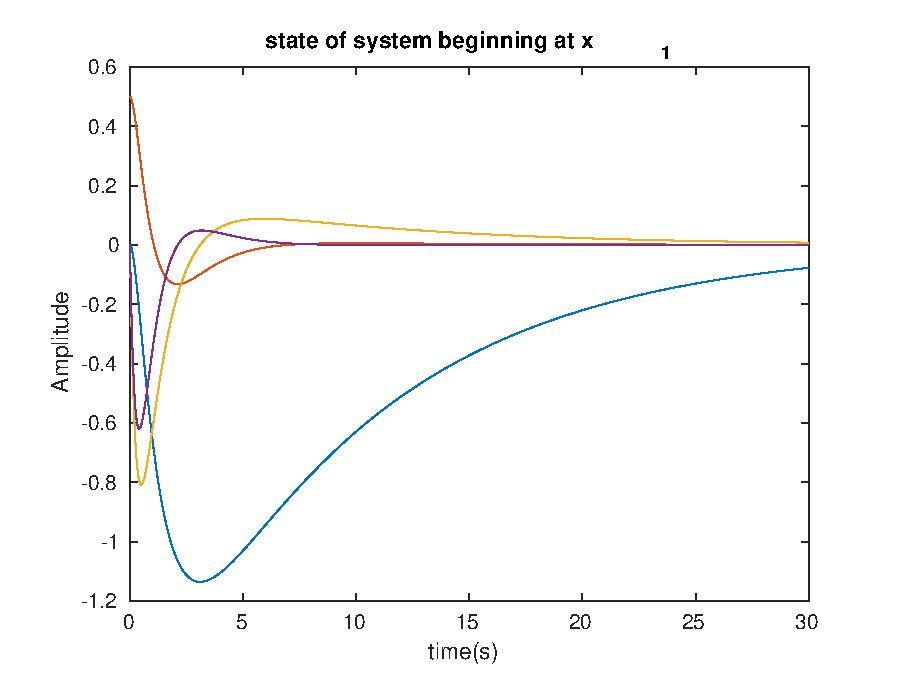
\includegraphics[width=\maxwidth{83.69292523833417em}]{figure_3.eps}
\end{center}


\vspace{1em}
\begin{matlabcode}
observer_tracker_position = observer_tracker(:,1)*39.3701;
% Plot of observer output against desired output
plot(t_1, observer_tracker_position)
hold on
plot(t_1,y_des)
hold off
title('Observed Position vs Desired Position')
ylabel('Position(m)')
xlabel('time(s)')
legend({'x̂', 'desired position'})
\end{matlabcode}
\begin{center}
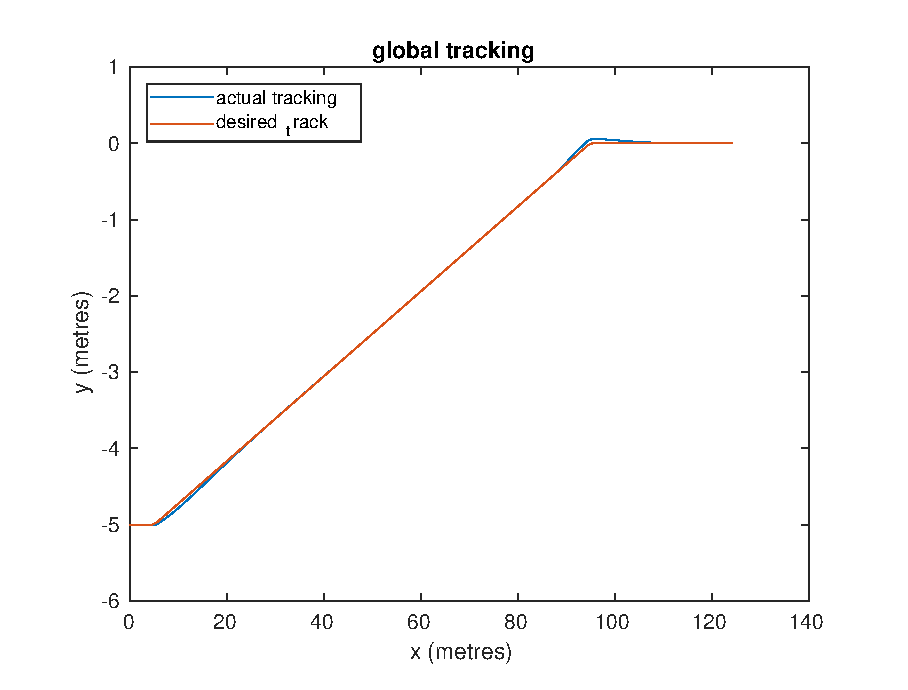
\includegraphics[width=\maxwidth{83.69292523833417em}]{figure_4.eps}
\end{center}


\vspace{1em}
\begin{par}
\begin{flushleft}
Controller System States vs Observer Estimates
\end{flushleft}
\end{par}

\begin{matlabcode}
% Plot of observer output against desired output
plot(t_1, controller_tracker_position)
hold on
plot(t_1, observer_tracker_position)
hold off
title('Controller Position State vs Observed Position')
ylabel('Position(m)')
xlabel('time(s)')
legend({'x_c', 'x̂'})
\end{matlabcode}
\begin{center}
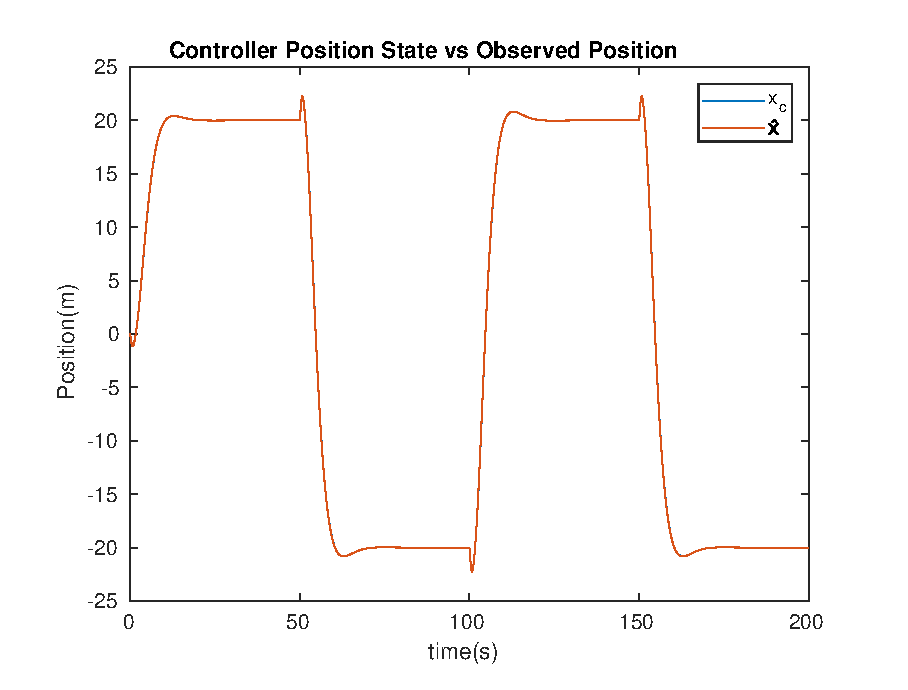
\includegraphics[width=\maxwidth{83.69292523833417em}]{figure_5.eps}
\end{center}


\vspace{1em}
\begin{par}
\begin{flushleft}
Error Plot: Controller System State (position) - Observer Estimate of Position
\end{flushleft}
\end{par}

\begin{matlabcode}
% Find the max error between the two plots
max_error = max(abs(controller_tracker_position - observer_tracker_position))
\end{matlabcode}
\begin{matlaboutput}
max_error = 0.0396
\end{matlaboutput}


\vspace{1em}
\begin{matlabcode}
% Plot the error over time
controller_observer_error = controller_tracker_position - observer_tracker_position;
plot(t_1, controller_observer_error)
title('Error between State & Observer vs time')
ylabel('Error(m)')
xlabel('time(s)')
\end{matlabcode}
\begin{center}
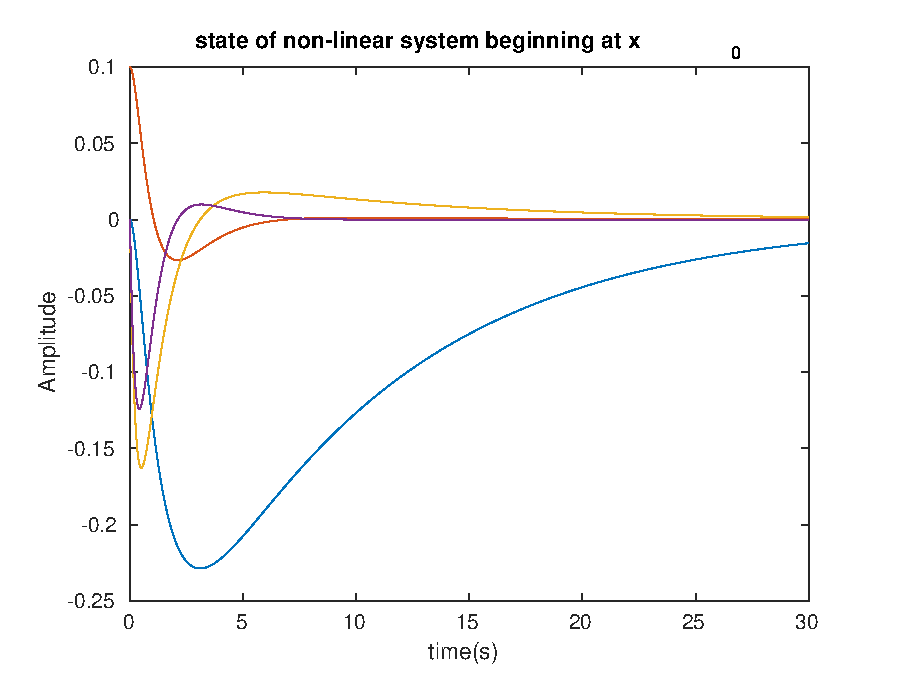
\includegraphics[width=\maxwidth{83.69292523833417em}]{figure_6.eps}
\end{center}


\begin{par}
\begin{flushleft}
Helper function for controller ODE45
\end{flushleft}
\end{par}

\begin{matlabcode}
function x_dot = tracking_controller (x, F, v, t)
xc = x(1);
phi = x(2);
xcdot = x(3);
phidot = x(4);

% constants in the system
gamma = 2;
alpha = 1;
beta = 1;
D = 1;
mu = 3;

% define parameters for y_des
freq=0.01;
offset=0;
amp=20;
duty=50;

% define y_des as a square wave function
y_des = offset+amp*square(2*pi*freq.*t,duty);
u = F + v*y_des;

divisor = ((gamma*alpha) - (beta*beta*cos(phi)*cos(phi)))^(-1);

x_dot = [xcdot;
        phidot;
        divisor*((u*alpha) - (beta*phidot*phidot*sin(phi)*alpha) - (alpha*mu*xcdot) + (beta*D*sin(phi)*cos(phi)));
        divisor*((u*beta*cos(phi)) - (beta*beta*phidot*phidot*sin(phi)*cos(phi)) - (beta*cos(phi)*mu*xcdot) + (gamma*D*sin(phi)))];


% divisor_1 = alpha / ((gamma*alpha) - (beta*beta*cos(phi)*cos(phi)));
% divisor_2 = (beta*cos(phi)) / ((gamma*alpha) - (beta*beta*cos(phi)*cos(phi)));

% x_dot = [xcdot;
%        phidot;
%        divisor_1*(u - (beta*phidot*phidot*sin(phi)) - (mu*xcdot) + ((beta*D*cos(phi)*sin(phi))/alpha));
%        divisor_2*(u - (beta*phidot*phidot*sin(phi)) - (mu*xcdot) + ((gamma*D*sin(phi)) / (beta*cos(phi))))];

end
\end{matlabcode}


\vspace{1em}
\begin{par}
\begin{flushleft}
Helper function for observer ODE45
\end{flushleft}
\end{par}

\begin{matlabcode}
function x_dot = tracking_controller_observer (x, K, v, t, K_0, controller_op, C)
xc = x(1);
phi = x(2);
xcdot = x(3);
phidot = x(4);

% constants in the system
gamma = 2;
alpha = 1;
beta = 1;
D = 1;
mu = 3;

% define parameters for y_des
freq=0.01;
offset=0;
amp=20;
duty=50;

% define y_des as a square wave function
y_des = offset+amp*square(2*pi*freq.*t,duty);
u = -K*x + v*y_des;

divisor = ((gamma*alpha) - (beta*beta*cos(phi)*cos(phi)))^(-1);

x_dot = [xcdot;
        phidot;
        divisor*((u*alpha) - (beta*phidot*phidot*sin(phi)*alpha) - (alpha*mu*xcdot) + (beta*D*sin(phi)*cos(phi)));
        divisor*((u*beta*cos(phi)) - (beta*beta*phidot*phidot*sin(phi)*cos(phi)) - (beta*cos(phi)*mu*xcdot) + (gamma*D*sin(phi)))];

error = K_0*(C*controller_op - C*x);
x_dot = x_dot + error;
% divisor_1 = alpha / ((gamma*alpha) - (beta*beta*cos(phi)*cos(phi)));
% divisor_2 = (beta*cos(phi)) / ((gamma*alpha) - (beta*beta*cos(phi)*cos(phi)));

% x_dot = [xcdot;
%        phidot;
%        divisor_1*(u - (beta*phidot*phidot*sin(phi)) - (mu*xcdot) + ((beta*D*cos(phi)*sin(phi))/alpha));
%        divisor_2*(u - (beta*phidot*phidot*sin(phi)) - (mu*xcdot) + ((gamma*D*sin(phi)) / (beta*cos(phi))))];

end
\end{matlabcode}

\end{document}
